% Build:  pdflatex lab_notebook.tex   (twice, for references)
\documentclass[11pt]{article}
\usepackage[margin=1in]{geometry}
\usepackage{amsmath,amssymb}
\usepackage[ruled,vlined,linesnumbered]{algorithm2e}
\usepackage{booktabs}
\usepackage{longtable}
\usepackage{array}
\usepackage{tikz}
\usepackage{xcolor}
\usepackage{listings}
\usepackage[T1]{fontenc}
\usepackage[utf8]{inputenc}
\usepackage[colorlinks=true,linkcolor=black,citecolor=black,urlcolor=blue]{hyperref}
\usetikzlibrary{arrows.meta,positioning,fit,backgrounds,calc}

\definecolor{ink}{HTML}{1F2328}
\definecolor{sub}{HTML}{57606A}
\definecolor{edge}{HTML}{D0D7DE}
\definecolor{panel}{HTML}{F6F8FA}
\definecolor{ideacol}{HTML}{8250DF}
\definecolor{codecol}{HTML}{0969DA}
\definecolor{notecol}{HTML}{1A7F37}
\definecolor{warm}{HTML}{BC4C00}

\lstset{
  basicstyle=\ttfamily\footnotesize, breaklines=true, breakatwhitespace=false,
  columns=fullflexible, keepspaces=true, frame=single, rulecolor=\color{edge},
  backgroundcolor=\color{panel}, xleftmargin=4pt, xrightmargin=4pt,
  aboveskip=6pt, belowskip=8pt, showstringspaces=false,
  literate={Ψ}{{$\Psi$}}1 {—}{{--}}1 {–}{{-}}1 {≤}{{$\le$}}1 {≥}{{$\ge$}}1 {×}{{$\times$}}1
}

\newcommand{\call}[1]{\textsc{#1}}

\title{\textbf{LabNotebook}\\[2mm]
\large Understanding-guided trajectory search for program evolution}
\author{Pantheon-Evolve \\ \small\texttt{pantheon.evolution.methods.LabNotebook}}
\date{September 2026}

\begin{document}
\maketitle

\begin{abstract}
\noindent LabNotebook is a two-level search. The inner level is SimpleTES: a short chain of
best-of-$k$ whole-program completions with no tools, no workspace and no self-scoring --- the
operator that won on cost in every campaign so far. The outer level is a scientist's loop whose
state is a \emph{lab notebook}: a bounded, sectioned prose understanding of the problem that the
model rewrites after every cycle; a history of every idea tried with the measured numbers next to
the digest; and a shelf of reference programs, each tagged with the idea that produced it. Each
cycle picks a parent, proposes $K$ distinct ideas, runs one short SimpleTES trajectory per idea
\emph{in parallel}, digests each trajectory against its idea, and updates the notebook. The
structural bet is that \textbf{an idea is scored by the best of a local search, not by one
implementation}. This document gives the algorithm, every prompt the method sends, exactly how an
idea is injected into a trajectory, how a trajectory is digested into understanding, and every
parameter with its default.
\end{abstract}

\section{Overview}

\begin{center}
\resizebox{\textwidth}{!}{%
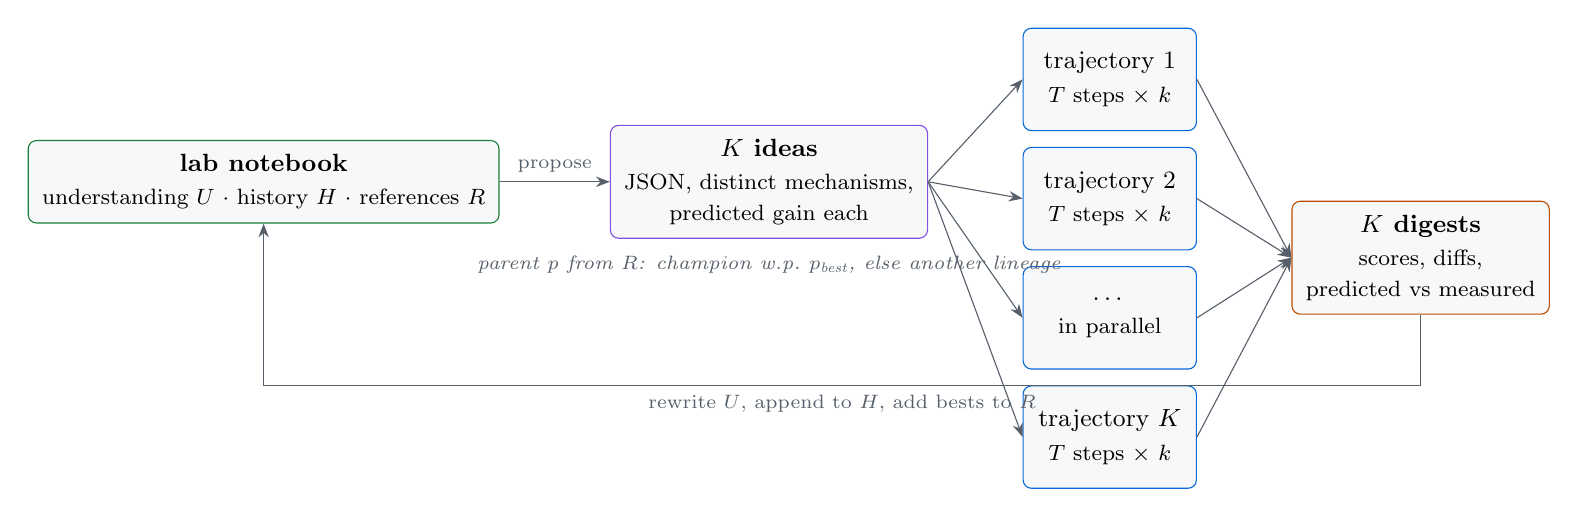
\begin{tikzpicture}[
  node distance=5mm and 8mm,
  box/.style={rounded corners=3pt, draw=edge, fill=panel, inner sep=5pt, align=center,
              font=\small},
  note/.style={box, draw=notecol, minimum width=40mm},
  idea/.style={box, draw=ideacol, minimum width=26mm},
  traj/.style={box, draw=codecol, minimum width=22mm, minimum height=13mm},
  ar/.style={-{Stealth[length=5pt]}, draw=sub},
]
\node[note] (nb) {\textbf{lab notebook}\\[1pt]\footnotesize understanding $U$ $\cdot$ history
  $H$ $\cdot$ references $R$};
\node[idea, right=14mm of nb] (ideas) {\textbf{$K$ ideas}\\[1pt]\footnotesize JSON, distinct
  mechanisms,\\ \footnotesize predicted gain each};
\node[traj, right=12mm of ideas, yshift=13mm] (t1) {trajectory 1\\[1pt]\footnotesize
  $T$ steps $\times$ $k$};
\node[traj, below=2mm of t1] (t2) {trajectory 2\\[1pt]\footnotesize $T$ steps $\times$ $k$};
\node[traj, below=2mm of t2] (t3) {\ldots\\[1pt]\footnotesize in parallel};
\node[traj, below=2mm of t3] (t4) {trajectory $K$\\[1pt]\footnotesize $T$ steps $\times$ $k$};
\node[box, draw=warm, right=12mm of t2, yshift=-7.5mm, minimum width=26mm] (dig)
  {\textbf{$K$ digests}\\[1pt]\footnotesize scores, diffs,\\ \footnotesize predicted vs
  measured};
\draw[ar] (nb) -- node[above,font=\scriptsize,text=sub]{propose} (ideas);
\foreach \t in {t1,t2,t3,t4} \draw[ar] (ideas.east) -- (\t.west);
\foreach \t in {t1,t2,t3,t4} \draw[ar] (\t.east) -- (dig.west);
\draw[ar] (dig.south) |- ++(0,-9mm) -| node[pos=0.25,below,font=\scriptsize,text=sub]
  {rewrite $U$, append to $H$, add bests to $R$} (nb.south);
\node[font=\scriptsize\itshape, text=sub, below=1mm of ideas] {parent $p$ from $R$: champion
  w.p.\ $p_{\text{best}}$, else another lineage};
\end{tikzpicture}}
\end{center}

\noindent The three arrows on the left are the method's own model calls (\call{Propose}, and
on the way back \call{Digest}$\times K$ and \call{Update}); the trajectories are SimpleTES steps
run by the framework's loop. One more call, \call{Understand}, writes the first notebook from the
seed before any cycle. All five are booked in the same LLM ledger as the operator's calls, so the
budget ceilings see the outer loop's spend.

\section{Algorithm}

\begin{algorithm}[H]
\SetAlgoLined
\DontPrintSemicolon
\KwIn{seed program $p_0$ with score $R(p_0)$; budget}
\KwOut{best measured program}
$U \gets \call{Understand}(\text{problem}, p_0)$ \tcp*{initial notebook, one call}
$H \gets [\,]$;\quad $R \gets [p_0]$;\quad $c \gets 0$\;
\While{budget remains}{
  $c \gets c + 1$\;
  $p \gets \call{SelectParent}(R)$ \tcp*{champion w.p.\ $p_{\text{best}}$, else another lineage}
  $I \gets \call{Propose}(U, H, p)$ \tcp*{$K$ ideas as JSON; retried once; blank fallback}
  \ForPar{$i \in I$}{
    chain $\gets [p]$\;
    \For{$s = 1 \ldots T$}{
      parents $\gets$ up to $n_{\text{insp}}$ best nodes of chain\;
      $C \gets$ \call{Operator}(idea $i$ + parents) \tcp*{$k$ candidates, one SimpleTES prompt}
      measure every $c \in C$;\quad chain $\gets$ chain $\cup$ \{best valid of $C$\}\;
    }
    $b_i \gets$ best valid candidate anchored on $i$ \tcp*{over ALL its candidates}
    $R \gets R \cup \{b_i\}$ \tcp*{tagged with $i$: its lineage}
  }
  \ForPar{$i \in I$}{
    $d_i \gets \call{Digest}(i,\ \text{all candidates of } i,\ \text{diff}(b_i, p),\
      \text{diff}(b_i, p_0),\ \text{predicted}_i)$\;
    $H \gets H + [(\text{numbers}_i, d_i)]$\;
  }
  $U \gets \call{Update}(U, \{d_i\}, \max R)$ \tcp*{same headings, cites the numbers}
}
\caption{LabNotebook. $U$ = the notebook (prose); $H$ = history rows (numbers + digest);
$R$ = reference programs; $K, T, k, n_{\text{insp}}, p_{\text{best}}$ in
Section~\ref{tab:params}. Trajectories advance concurrently, bounded by the loop's worker count.}
\end{algorithm}

\paragraph{Parent selection.} References are sorted by score. With probability
$p_{\text{best}}$ the champion is the parent. Otherwise the candidates are the references whose
\emph{lineage} (the idea they came from, \texttt{anchor\_id}) differs from the champion's; the
top half of those by score forms the pool and one is drawn uniformly. A search that always
builds on its champion collapsed to hill-climbing on Erd\H{o}s (the warm-start ablation); the
30\% lineage draw is the counterweight.

\section{The five model calls}

Every call has a system prompt (fixed text, below verbatim) and a user prompt assembled from the
run's state. The operator call uses \emph{no} system message --- that is SimpleTES's own
convention and is kept so the inner loop remains SimpleTES.

\begin{center}\small
\begin{tabular}{llll}
\toprule
call & fires & per cycle & output parsed as \\
\midrule
\call{Understand} & once, before cycle 1 & --- & markdown notebook (6 headings) \\
\call{Propose} & start of every cycle & 1 & JSON list of $K$ ideas \\
\call{Operator} & every trajectory step & $K\,T$ prompts\footnotemark &
  one program per candidate \\
\call{Digest} & end of every cycle, per idea & $K$ (in parallel) & JSON object \\
\call{Update} & end of every cycle & 1 & markdown notebook (same headings) \\
\bottomrule
\end{tabular}
\end{center}
\footnotetext{Each prompt asks for $k$ candidates. OpenRouter ignores the \texttt{n} parameter, so
a $k$-candidate prompt becomes $k$ requests; the search is identical, the call count is $k\times$.}

\subsection{\call{Understand} --- the first notebook}

\noindent\textbf{System prompt} (verbatim):
\begin{lstlisting}
You are a research scientist keeping a lab notebook on an optimisation problem. Write a compact, factual account under EXACTLY these markdown headings, in this order: ## Problem structure / ## Current best approach and its performance / ## What limits the score / ## What has worked (with numbers) / ## What has not worked (with numbers) / ## Open directions. Be specific about mechanisms and quantities. No code. Stay under 700 words.
\end{lstlisting}

\noindent\textbf{User prompt} (template; \texttt{\{\}} marks a filled slot):
\begin{lstlisting}
# Problem
{objective.md, the task statement given to every method}

# Seed program (score {seed score}; metrics: {k=v, ... every scalar metric})
```
{seed source, complete -- never truncated}
```

Write the initial notebook.
\end{lstlisting}
The reply is stored as $U$ verbatim (an empty reply becomes the placeholder
\texttt{(no understanding yet)}).

\subsection{\call{Propose} --- $K$ ideas}

\noindent\textbf{System prompt} (verbatim):
\begin{lstlisting}
You are a research scientist proposing the next experiments on an optimisation problem, using your lab notebook and the record of what has already been tried. Propose exactly K ideas that target DIFFERENT mechanisms from each other. Each idea must be concrete enough that a programmer can implement it without asking a question, and specific enough to be wrong. Do not repropose something the record shows was tried and failed unless you say what would be done differently and why. Reply with JSON only: a list of objects {"title": "<6 words>", "idea": "<3-6 sentences>", "predicted_gain": <number: expected change in combined_score, may be small or negative>}.
\end{lstlisting}

\noindent\textbf{User prompt:}
\begin{lstlisting}
# Problem
{objective}

# Lab notebook
{U, the current notebook}

# Record of ideas tried
| cycle | idea | parent | best | delta | predicted | adherence | outcome |
|---|---|---|---|---|---|---|---|
| 1 | Exact LP radii inner loop | 1.80452 | 2.577589619978106 | +0.77307 | +0.02000 | 0.95 | Best score improved from ... |
...  (the last 24 rows)

Lessons recorded:
- {lesson from each digest, last 12}

# Parent program for this cycle (score {R(p)}; metrics: {...})
```
{parent source, complete}
```

Propose exactly K={K} ideas as JSON.
\end{lstlisting}
The reply is parsed as a JSON list (fences and surrounding prose are tolerated). Each element
needs a non-empty \texttt{idea}; \texttt{title} defaults to the idea's first 40 characters and
\texttt{predicted\_gain} to 0 when missing or non-numeric. An unparseable reply is retried once;
if both fail the cycle runs one blank idea (``Improve the program in whatever way the evidence
suggests'') rather than stalling. Each accepted idea is stored as a \texttt{kind="idea"}
individual so that every program it produces can point at it.

\subsection{\call{Operator} --- one trajectory step (SimpleTES's prompt, idea injected)}
\label{sec:operator}

No system message. The prompt is SimpleTES's own generation template, reproduced from the
authors' source; LabNotebook contributes only the \emph{instruction} that heads it. For a seed
without EVOLVE-BLOCK markers (Erd\H{o}s, circle packing) the whole file is regenerated:

\begin{lstlisting}
{INSTRUCTION -- see section 4}

## Reference programs (2 of them), best first        <- step 2 onward; step 1 has one parent:
### reference 1 (combined_score = 2.5776)               "## Current program `solution.py` (...)"
```python
{full source of the trajectory's best node}
```
### reference 2 (combined_score = 1.8045)
```python
{full source of the next node}
```

Write a NEW program, better than all of them. Prefer an approach none of them takes; combine what works where that helps.

## Recurring failures to avoid                       <- only when this trajectory has failures
- {reason} (x{count})

Reply with the complete new `solution.py` in one fenced code block.
\end{lstlisting}

For a seed with markers (AHC039, a 43\,KB C++ program) only the block between the markers is
regenerated, with the authors' template verbatim:

\begin{lstlisting}
Task: {INSTRUCTION}

Generation instruction (must follow exactly):
1) Only the code between `// EVOLVE-BLOCK-START` and `// EVOLVE-BLOCK-END` is extracted.
2) The final program is reconstructed as EXACT_PREFIX + evolved_block + EXACT_SUFFIX.
3) Keep marker lines exactly as written.
4) Return one C++ code block that includes both EVOLVE-BLOCK markers.

EXACT_PREFIX (kept unchanged):
```cpp
{prefix}
```

EXACT_SUFFIX (kept unchanged):
```cpp
{suffix}
```

=== REFERENCE SOLUTIONS ===

[SAMPLED INSPIRATIONS] (2 solutions sampled for detailed reference)
Learn from these specific implementations - study their patterns and techniques.

--- Inspiration 1 ---
Score: {score}
Metrics:
  {every metric}
Code:
```cpp
{full program}
```
...
[FAILURE PATTERNS] (common errors to avoid)
- {reason} (x{count})

=== GENERATION STRATEGY ===
- Prioritize NOVEL approaches not yet seen in the elite pool
- Only refine existing approaches if you identify clear improvement potential
- Combine insights from multiple solutions when beneficial
- Avoid the listed failure patterns

Generate an improved solution with higher score:
\end{lstlisting}

The reply's last fenced block is the program (models often restate the original first; taking
the first block would silently resubmit the parent). A reply without a code block is re-rolled
once. Temperature 1.0, \texttt{max\_tokens} 32768 unless \texttt{--max-output-tokens} raises it
(64000 on Erd\H{o}s and packing, where deepseek-v4-flash needs $\sim$26k tokens of thinking
before it writes anything).

\subsection{\call{Digest} --- one idea's write-up}

\noindent\textbf{System prompt} (verbatim):
\begin{lstlisting}
You are a research scientist writing up one experiment in a lab notebook. You are given the idea that was tested, every candidate program's score along its search trajectory, the best program's diff against its parent and against the original seed, and the predicted gain. Reply with JSON only: {"outcome": "<one sentence: what happened, with the numbers>", "why": "<2-4 sentences: the mechanism you infer for the result>", "adherence": <0-1: how faithfully the trajectory actually pursued the idea>, "lesson": "<one sentence a future proposer should know>"}
\end{lstlisting}

\noindent\textbf{User prompt:}
\begin{lstlisting}
# Problem
{objective}

# Idea tested
{title}
{idea text}
predicted gain: {+0.02000}

# Trajectory (parent score {R(p)})
- candidate 7f60aa3b: score=2.2488
- candidate b45de5c3: score=2.577589619978106
- candidate 011c2794: score=invalid  error: {evaluator's error, first 120 chars}
- candidate 2cd63e42: score=2.51
                                        <- EVERY candidate anchored on the idea, in creation
                                           order, not only the ones committed to the chain
best: {best score}  delta vs parent: {+0.77307}

# Best program's diff vs parent
```diff
{unified diff, 2 lines of context, capped at 6000 chars}
```

# Best program's diff vs original seed
```diff
{unified diff vs the seed; "(same as parent diff)" in cycle 1}
```

# Failures during the trajectory              <- only if the operator reported failures
- {reason} (x{count})

Write the digest as JSON.
\end{lstlisting}
Parsed as a JSON object; retried once if \texttt{outcome} is empty. \texttt{adherence} is
clamped to $[0,1]$; text fields are capped (outcome 300, why 600, lesson 300 chars). The
\emph{numbers} of the history row --- parent score, best score, delta, predicted gain, candidate
count --- are computed by the method, not by the model, and are written whether or not the
prose parsed.

\subsection{\call{Update} --- rewriting the notebook}

\noindent\textbf{System prompt} (verbatim):
\begin{lstlisting}
You are a research scientist revising your lab notebook after a batch of experiments. Rewrite the notebook under EXACTLY the same headings, integrating the new results. Cite the measured numbers; where a result contradicts an earlier belief, change the belief and say what changed it. Keep what is still true, drop what is superseded. No code. Stay under 700 words.
\end{lstlisting}

\noindent\textbf{User prompt:}
\begin{lstlisting}
# Problem
{objective}

# Notebook before this cycle
{U}

# This cycle's experiments (cycle {c}, parent score {R(p)})
### {title} (predicted +0.02000, measured +0.77307, adherence 0.95)
outcome: {...}
why: {...}
lesson: {...}

### {next idea} ...

# Best score so far: {max over references}

Rewrite the notebook.
\end{lstlisting}
A non-empty reply replaces $U$; an empty one leaves the previous notebook in place.

\section{How an idea is injected into a trajectory}
\label{sec:inject}

\paragraph{The instruction.} Every trajectory step's prompt begins with this text, built fresh
at each step from the idea the trajectory belongs to:
\begin{lstlisting}
{objective}

## The ONE idea this trajectory tests: {title}
{idea text}

Every candidate you write must implement or advance THIS idea on the reference program(s) below. Keep everything the idea does not touch intact; do not switch to an unrelated improvement.
\end{lstlisting}
It lands as the first block of the whole-file prompt, and as the \texttt{Task:} line of the
EVOLVE-BLOCK prompt (Section~\ref{sec:operator}). Nothing else in the operator's prompt is
changed.

\paragraph{Why every step, not just the first.} A prefix on step 1 only would drift: by step 2
the prompt shows the step-1 winner as a reference and SimpleTES's own strategy text asks for
``novel approaches'', and the trajectory would revert to generic improvement while still wearing
the idea's name. Re-stating the idea at every step keeps ``best of this idea's trajectory'' an
honest measurement of the idea.

\paragraph{The trajectory is its own chain.} Each idea gets a fresh SimpleTES chain seeded with
the cycle's parent only. Inspirations for a step are drawn from \emph{that chain} (its best
node first, then SimpleTES's stratified draw) --- never from other trajectories or from the
references --- so what a trajectory learns from is the parent plus its own committed winners.
Failure patterns are per trajectory for the same reason. After each step exactly one child, the
best valid of the $k$, joins the chain; the others stay in the store and still count for the
digest.

\paragraph{Provenance.} Every candidate is created with \texttt{anchor\_id} = the idea's
individual id, in addition to its code parents. That edge is what lets the digest collect
\emph{all} candidates of an idea (committed or not), lets a reference program remember which
idea produced it (the lineage used by parent selection), and lets the run's store be audited
afterwards: which idea each program was testing is recorded, not inferred.

\paragraph{A tension worth knowing.} The operator's closing line --- \emph{``Prefer an approach
none of them takes''} --- is SimpleTES's and is kept verbatim so the inner loop stays SimpleTES.
It pulls mildly against ``pursue THIS idea''. The instruction leads the prompt and is
repeated every step; the digest's \texttt{adherence} field is the check on whether the pull
won. In the smoke run three of four trajectories were rated 0.90--0.95.

\section{How a trajectory becomes understanding}

Three artefacts, in order:

\begin{enumerate}
\item \textbf{The measurement of the idea.} $b_i$ = the best \emph{valid, full-fidelity} candidate
  among everything anchored on idea $i$. Its score, $\Delta = R(b_i) - R(p)$, the predicted gain,
  and the candidate count are the row's numbers. If no candidate was valid the row records
  \texttt{invalid} and $\Delta = 0$; $b_i$ joins the references only if valid. Ties in score
  are routine (two candidates of one prompt, two invalid ones) and are broken by a key-based
  maximum.
\item \textbf{The digest.} The \call{Digest} prompt receives the idea, every candidate's score and
  evaluator error, the best program's diff against the parent (what this idea changed) and
  against the seed (how far the lineage has drifted), and the prediction. Its four fields are
  merged into the same history row.
\item \textbf{The notebook rewrite.} \call{Update} receives the previous $U$, all $K$ digests of the
  cycle with their numbers, and the best score so far, and produces the new $U$ under the same
  six headings with the same 700-word cap. The cap and the fixed headings are what stop the
  notebook from either growing without bound or forgetting.
\end{enumerate}

\noindent The history is then rendered into the next \call{Propose} prompt as the table in
Section~3.2 (last 24 rows) plus the last 12 lessons. The numbers come from the method; the prose
comes from the model; both are always shown together, so a later proposal cannot cite the
story without the measurement beside it. The predicted-vs-measured column is also the run's
cheapest calibration signal: in the smoke run the LP inner loop was predicted $+0.02$ and
measured $+0.77$, and the digest's own lesson was that a cheap exact inner loop ``can unlock far
more gain than its direct score delta suggests''.

\section{A real cycle, from the smoke run}

Circle packing ($n=26$), seed 1.804524, deepseek-v4-flash, $K=4$, $T=2$, $k=2$.

\paragraph{Cycle 1 ideas and digests}
\begin{center}\small
\begin{tabular}{@{}lrrr>{\raggedright\arraybackslash}p{58mm}@{}}
\toprule
idea & predicted & measured $\Delta$ & adherence & lesson (abridged) \\
\midrule
Exact LP radii inner loop & $+0.020$ & $+0.773$ & 0.95 & a cheap exact inner loop unlocks far
  more than its own delta \\
Multi-start SLSQP & $+0.650$ & $+0.830$ & --- & (digest unparsed; numbers kept) \\
Penalty-barrier annealing & $+0.400$ & $+0.816$ & 0.90 & predictions underestimate global
  search; many restarts pay \\
CMA-ES + SLSQP polish & $+0.500$ & $+0.807$ & 0.90 & needs stricter feasibility to reach
  the exact record \\
\bottomrule
\end{tabular}
\end{center}

\paragraph{The rewritten notebook, ``What has worked'' (excerpt)}
\begin{itemize}\itemsep1pt\small
  \item Exact LP radii inner loop on the original ring centres lifted the score from
    \textbf{1.804524} to \textbf{2.2488} (+0.4443) --- the old fixed-centre radii were severely
    suboptimal.
  \item Multi-start SLSQP with random centre seeds, using the LP inner loop, improved the best
    to \textbf{2.5776} and later to \textbf{2.634292}.
  \item Penalty-barrier annealing with SLSQP polish reached \textbf{2.6206} (+0.8161 over seed).
  \item CMA-ES exploration + LP/SLSQP polish reached \textbf{2.6111} (+0.8066).
\end{itemize}
and under ``What limits the score'': \emph{``Near the optimum the contact graph is almost
jammed: moving one centre to enlarge a circle typically forces several neighbouring circles to
shrink \ldots the best found configuration still lacks the tiny global rearrangement that would
close the last 0.00169.''}

\paragraph{Cycle 2} started from the CMA-ES lineage (2.6111) rather than the champion --- the
lineage draw fired --- and proposed four new mechanisms with predictions now calibrated to being
near the record: LP-duality gradient ascent on centres ($+0.0007$), contact-graph simulated
annealing ($+0.0012$), surrogate-based Bayesian optimisation ($+0.0009$), augmented Lagrangian
with exact LP inner solve ($+0.0004$).

\section{Parameters}
\label{tab:params}

\begin{center}\small
\begin{tabular}{@{}>{\raggedright\arraybackslash}p{40mm}>{\raggedright\arraybackslash}p{36mm}>{\raggedright\arraybackslash}p{80mm}@{}}
\toprule
parameter & default & meaning \\
\midrule
\texttt{ideas\_per\_cycle} ($K$) & 4 & ideas proposed, and trajectories run, per cycle \\
\texttt{steps\_per\_trajectory} ($T$) & 2 & SimpleTES steps per trajectory \\
\texttt{k\_candidates} ($k$) & 2 & candidates per step (one prompt; best-of-$k$ commits) \\
\texttt{num\_inspirations} ($n_{\text{insp}}$) & 2 & chain nodes shown as references per step \\
\texttt{p\_best\_parent} ($p_{\text{best}}$) & 0.7 & probability a cycle starts from the
  champion; otherwise a different lineage \\
\texttt{history\_window} & 24 & history rows shown to \call{Propose} (plus last 12 lessons) \\
\texttt{score\_key}, \texttt{valid\_key} & \texttt{combined\_score}, \texttt{validity} &
  the metric read as the score; validity $>0$ required \\
\texttt{seed} & 0 & RNG seed for parent and inspiration draws \\
\midrule
notebook headings & 6, fixed & Problem structure $\cdot$ Current best approach $\cdot$ What
  limits the score $\cdot$ What has worked $\cdot$ What has not worked $\cdot$ Open directions \\
notebook length & $\le 700$ words & stated in \call{Understand} and \call{Update} \\
diff cap & 6000 chars & each of the two diffs in the \call{Digest} prompt \\
retries & 1 & \call{Propose} on unparseable JSON; \call{Digest} on empty outcome; operator on a
  reply without a code block \\
\midrule
operator & \texttt{Upstream}\-\texttt{Completion}\-\texttt{Variator} & SimpleTES's own; no system message \\
\texttt{max\_tokens} & 32768 & or \texttt{--max-output-tokens} (64000 on Erd\H{o}s/packing) \\
\texttt{reasoning\_max\_tokens} & none & cap on a reasoning model's thinking, if passed \\
temperature & 1.0 & operator default \\
model & the run's \texttt{--model} & the method's own calls use the operator's model, tokens
  and reasoning cap \\
\midrule
bench setting & \texttt{--workers 4} & concurrency = trajectories advancing at once \\
\bottomrule
\end{tabular}
\end{center}

\paragraph{Budget arithmetic.} Per cycle, with $K=4$, $T=2$, $k=2$ behind a gateway that
ignores \texttt{n}: $1$ (\call{Propose}) $+ K\,T\,k = 16$ (operator) $+ K = 4$ (\call{Digest})
$+ 1$ (\call{Update}) $= 22$ LLM calls and $K\,T\,k = 16$ evaluator calls, plus one
\call{Understand} at the start. A 160-call arm runs $\sim$7 cycles; a 480-call arm $\sim$21.
Wall-clock per cycle with deepseek-v4-flash at 64k output was $\sim$25 minutes, most of it the
three sequential outer calls.

\paragraph{Guards and persistence.} Every model call the method makes is wrapped: an exception
or empty reply degrades (blank idea, empty digest prose, unchanged notebook) rather than ending
the run. State (\,$U$, $H$, $R$, ideas, trajectories, cycle\,) is checkpointed with the store;
on resume, batches that were in flight are dropped and each trajectory continues from the step
it had completed, so a preempted container costs the open step and nothing else.

\section{Interim results}

At the time of writing the flash-model campaign is still running (all figures are lower bounds
for unfinished arms). Circle packing: all three LabNotebook arms reached the published record
2.635983 exactly, within 64--82 of their 160 calls; the previous wave's best was one arm in nine.
Erd\H{o}s: the best method mean of the four ($\Psi$ 0.3812--0.3827), still above the 0.380909
record --- the basin holds for every method. AHC039: 3707--3720 at half budget against
finished arms at 3714--3730; not yet comparable. On every task LabNotebook's token spend is the
lowest of the four methods. The ablation that would attribute the packing result --- plain
SimpleTES vs LabNotebook vs LabNotebook with random ideas and no notebook, same budget --- has
not been run.

\vfill
\noindent\footnotesize Source: \texttt{pantheon/evolution/methods/lab\_notebook.py}\\
Operator: \texttt{methods/simpletes.py}, \texttt{variators/completion.py}\\
Bench wiring: \texttt{run\_bench.py --method lab\_notebook} $\cdot$ companion:
\texttt{hypothesis\_bandit.pdf}
\end{document}
